% Template for fig_results.tex; @...@ fields are filled from model v0.7 by gen_fig.py.
\documentclass[border=4pt]{standalone}
\usepackage[T1]{fontenc}
\usepackage[scaled=0.92]{helvet}
\renewcommand\familydefault{\sfdefault}
\usepackage{pgfplots}
\usepackage{sansmath}\sansmath
\pgfplotsset{compat=1.17}
% Team palette (docs/style-guide.md)
\definecolor{ink}{HTML}{26313A}
\definecolor{oxide}{HTML}{1E5245}
\definecolor{sand}{HTML}{F6EFDF}
\definecolor{band}{HTML}{F3F5F2}
\definecolor{muted}{HTML}{6B7780}
\definecolor{rule}{HTML}{C9CFC9}
\definecolor{amber}{HTML}{9A6A14}
\definecolor{brick}{HTML}{A33B2B}

\begin{document}
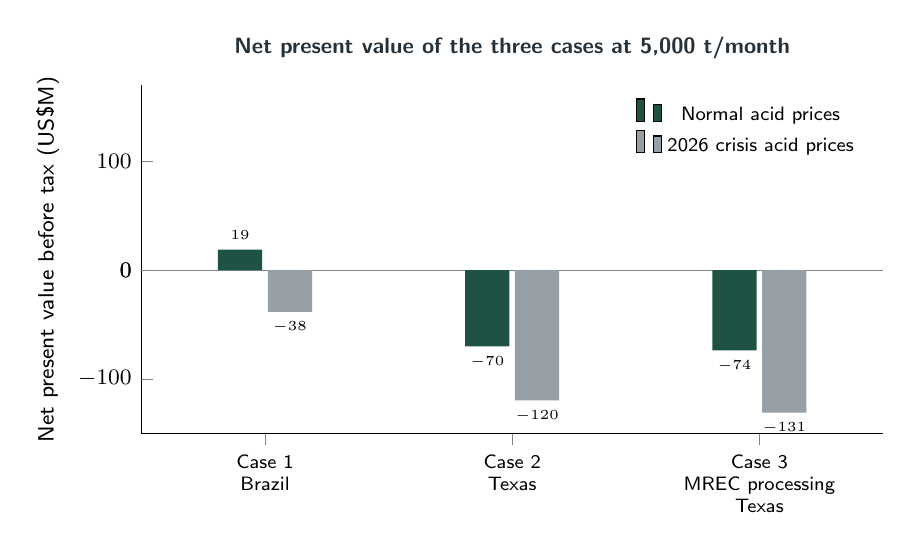
\begin{tikzpicture}[font=\footnotesize\sffamily]
\begin{axis}[name=a, width=11cm, height=6cm, ybar, bar width=16pt, ymin=-150, ymax=170,
  xtick={0,1,2}, xticklabels={Case 1\\Brazil,Case 2\\Texas,Case 3\\MREC processing\\Texas}, xticklabel style={align=center, font=\scriptsize\sffamily},
  enlarge x limits=0.25, ylabel={Net present value before tax (US\$M)}, axis lines*=left,
  legend style={draw=none, at={(0.98,0.98)}, anchor=north east, font=\scriptsize\sffamily},
  nodes near coords, nodes near coords style={font=\tiny\sffamily, /pgf/number format/.cd, fixed, precision=0},
  title={\textbf{Net present value of the three cases at 5,000 t/month}}, title style={font=\footnotesize\sffamily, color=ink},
  extra y ticks={0}, extra y tick style={grid=major, grid style={draw=ink!60}}]
\addplot[fill=oxide, draw=none] coordinates {(0,19.0) (1,-70.1) (2,-73.6)};
\addplot[fill=muted!70, draw=none] coordinates {(0,-38.2) (1,-119.7) (2,-130.9)};
\legend{Normal acid prices, 2026 crisis acid prices}
\end{axis}
\end{tikzpicture}
\end{document}
